\documentclass[a4paper, 12pt]{article}

%%% Работа с русским языком
\usepackage{cmap}					% поиск в PDF
\usepackage{mathtext} 				% русские буквы в формулах
\usepackage[T2A]{fontenc}			% кодировка
\usepackage[utf8]{inputenc}			% кодировка исходного текста
\usepackage[russian]{babel}	% локализация и переносы

%%% Дополнительная работа с математикой
\usepackage{amsmath,amsfonts,amssymb,amsthm,mathtools} % AMS
\usepackage{icomma} % "Умная" запятая: $0,2$ --- число, $0, 2$ --- перечисление

%% Номера формул
%\mathtoolsset{showonlyrefs=true} % Показывать номера только у тех формул, на которые есть \eqref{} в тексте.

%% Шрифты
\usepackage{euscript}	 % Шрифт Евклид
\usepackage{mathrsfs} % Красивый матшрифт

%% Поля
\usepackage[left=2cm,right=2cm,top=2cm,bottom=2cm,bindingoffset=0cm]{geometry}

%% Русские списки
\usepackage{enumitem}
\makeatletter
\AddEnumerateCounter{\asbuk}{\russian@alph}{щ}
\makeatother

%%% Работа с картинками
\usepackage{graphicx}  % Для вставки рисунков
\graphicspath{{images/}{images2/}}  % папки с картинками
\setlength\fboxsep{3pt} % Отступ рамки \fbox{} от рисунка
\setlength\fboxrule{1pt} % Толщина линий рамки \fbox{}
\usepackage{wrapfig} % Обтекание рисунков и таблиц текстом

%%% Работа с таблицами
\usepackage{array,tabularx,tabulary,booktabs} % Дополнительная работа с таблицами
\usepackage{longtable}  % Длинные таблицы
\usepackage{multirow} % Слияние строк в таблице

%% Красная строка
\setlength{\parindent}{2em}

%% Интервалы
\linespread{1}
\usepackage{multirow}

%% TikZ
\usepackage{tikz}
\usetikzlibrary{graphs,graphs.standard}

%% Верхний колонтитул
\usepackage{fancyhdr}
\pagestyle{fancy}

%% Перенос знаков в формулах (по Львовскому)
\newcommand*{\hm}[1]{#1\nobreak\discretionary{}
	{\hbox{$\mathsurround=0pt #1$}}{}}

%% Мои дополнения
\usepackage{float} %Добавляет возможность работы с командой [H] которая улучшает расположение на странице
\usepackage{gensymb} %Красивые градусы
\usepackage{graphicx}               % Импорт изображений
\usepackage{caption} % Пакет для подписей к рисункам, в частности, для работы caption*

% подключаем hyperref (для ссылок внутри  pdf)
\usepackage[unicode, pdftex]{hyperref}

%%% Теоремы
\theoremstyle{plain}                    % Это стиль по умолчанию, его можно не переопределять.
\renewcommand\qedsymbol{$\blacksquare$} % переопределение символа завершения доказательства

\newtheorem{theorem}{Теорема}[section] % Теорема (счетчик по секиям)
\newtheorem{proposition}{Утверждение}[section] % Утверждение (счетчик по секиям)
\newtheorem{definition}{Определение}[section] % Определение (счетчик по секиям)
\newtheorem{corollary}{Следствие}[theorem] % Следстиве (счетчик по теоремам)
\newtheorem{problem}{Задача}[section] % Задача (счетчик по секиям)
\newtheorem*{remark}{Примечание} % Примечание (можно переопределить, как Замечание)
\newtheorem{lemma}{Лемма}[section] % Лемма (счетчик по секиям)
% % \newcommand{\eqdef}{\stackrel{\mathrm{def}}{=}}
% \newcommand{\ryad}{\sum\limits^{\infty}_{k = 0}}

% \newcommand{\R}{\mathbb{R}}
% \newcommand{\N}{\mathbb{N}}
% \newcommand{\series}{\sum\limits_{k=1}^{\infty}}
% \newcommand{\useries}{\sum\limits_{k=1}^{\infty} u_k}
% \newcommand{\useriesl}{\sum\limits_{k=1}^{\infty} u_k < \infty}
% \newcommand{\useriese}{\sum\limits_{k=1}^{\infty} u_k = \infty}
% \newcommand{\auseries}{\sum\limits_{k=1}^{\infty} |u_k|}
% \newcommand{\auseriesl}{\sum\limits_{k=1}^{\infty} |u_k| < \infty}
% \newcommand{\auseriese}{\sum\limits_{k=1}^{\infty} |u_k| = \infty}
% \newcommand{\sn}{\sum\limits_{k=1}^{n} u_k}

% \renewcommand {\ge}{\geqslant}
% \renewcommand {\le}{\leqslant}
% \renewcommand {\geq}{\geqslant}
% \renewcommand {\leq}{\leqslant}
% \renewcommand {\epsilon}{\varepsilon}

\begin{document}
	
	\newcommand{\HRule}{\rule{\linewidth}{0.7mm}} % Defines a new command for the horizontal lines, change thickness here
	
	\begin{center}
		\large\textbf{Московский Физико-Технический Институт}\\ % Name of your university/college
		\large\textbf{(государственный университет)}
	
		\vfill
		
		\Large Лабораторная работа по курсу общей физики № *labnum*\\[0.5cm] % Preambule of your document title
		
		
		\HRule
		\\[0.4cm]
		{ \huge \bfseries *name of your labwork*}% Title of your document
		\\[0.4cm] 
		\HRule
		\\[0.5cm]
		
		\ \\
	\textbf{\large Автор:} \\	
	\large *your name* *groupname*\\ % Your name and something more, your group num for example
		\vfill
		\hspace*{-0.8 cm}
\includegraphics[width=100 pt]{frkt_logo}\\ % logo of your  company/university/college
		\large Долгопрудный, 2021 % location and year
	\end{center}

\newpage
\setcounter{page}{2}
\fancyfoot[c]{\thepage}
\fancyhead[L] {Работа № *labnum*} % some information in page header
\fancyhead[R]{}
	
	\section{Подготовка.}
	
	\noindent \textbf{В работе используются:} генератор импульсов, электронное реле, магазин сопротивлений, магазин емкостей, индуктивность, осциллограф, измеритель LCR.
	
	\noindent \textbf{Цель работы:} исследование зависимости периода свободных колебаний контура от емкости, зависимость логарифмического декремента затухания от сопротивления, определить критическое сопротивление и добротность контура, пронаблюдать затухающие колебания на фазовой плоскости.
	
	\hfill \break
	
	\noindent \textbf{Схема установки.}
	
	\begin{figure} [h!]
		\centering
		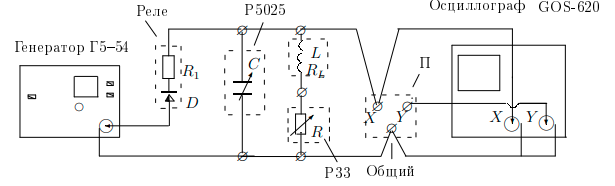
\includegraphics[scale = 0.75]{Схема установки для исследования свободных колебаний.png}
		\caption{Схема установки для исследования свободных колебаний}
	\end{figure}
	
	\hfill \break
	
	\noindent \textbf{Расчетные формулы.}
	
	\noindent Период колебательного контура.
	\begin{equation}
	T = 2 \pi \sqrt{LC}
	\end{equation}
	
	\noindent Частота колебательного контура.
	\begin{equation}
	\nu_0 = \frac{1}{2 \pi \sqrt{LC}}
	\end{equation}
	
	\noindent Критическое сопротивление.
	\begin{equation}
	R_{\text{кр}} = 2 \sqrt{\frac{L}{C}}
	\end{equation}
	
	\noindent Логарифмический декремент затухания.
	\begin{equation}
	\Theta = \frac{1}{n} \ln \frac{U_k}{U_{k + n}}
	\end{equation}
	
	\noindent Добротность.
	\begin{equation}
	Q = 2 \pi \frac{W}{\Delta W_T} = \frac{W}{\Delta W} = \frac{\pi}{\gamma T} = \frac{\omega_0 L}{R} = \frac{1}{\omega_0 CR} = \frac{1}{R} \sqrt{\frac{L}{C}}
	\end{equation}
	
	\newpage
	
	\section{Обработка данных.}
	
	\noindent Экспериментальным путем измерили период колебаний, при $R = 0$ $T = 340$ мкс; тогда частота колебаний составляет $\nu \approx 2941.18 Hz \approx 3 ~ \text{кГц} $.
	
	\hfill
	
	\noindent Используя формулу Томсона, вычислим индуктивность
	\begin{equation*}
		T = 2 \pi \sqrt{LC} \Rightarrow L = \frac{1}{C} \left(\frac{T}{2 \pi} \right)^2 = \frac{1}{2 \cdot 10^{-8}} \frac{3.4^2 \cdot 10^{-8}}{4 \pi^2} \approx 146.55 ~ \text{мГн}
	\end{equation*}
	
	\noindent Измерим индуктивность при помощи прибора ТЕТРОН-RLC200. Полученное значение -- $L = 143.47$ мГн.
	
	\noindent Примем расчетную погрешность 4\%; погрешность вычисления индуктивности $(\pm 5.74 ~ \text{мГн})$.
	
	\hfill
	
	\noindent \textbf{Вывод:} Таким образом, приходим к выводу, что полученные значения совпадают в пределах погрешности.
	
	\hfill
	
	\noindent Измерим зависимость $T^2(C)$; построим график данной зависимости.
	
	\begin{table}[h!]
		\begin{center}
			\begin{tabular}{|c|c|c|c|c|c|} \hline
				$C$ ($10^{-2}$ мкФ)   & 1     & 2      & 4      & 7      & 9 \\ \hline
				$T^2$ ($10^3$ мкс$^2$) & 57.6  & 115.6  & 230.4  & 409.6  & 518.4  \\ \hline
			\end{tabular}
		\end{center}
	\end{table}

	\noindent По графику проверим справедливость формулы Томсона.
	
	\begin{figure} [h!]
		\centering
		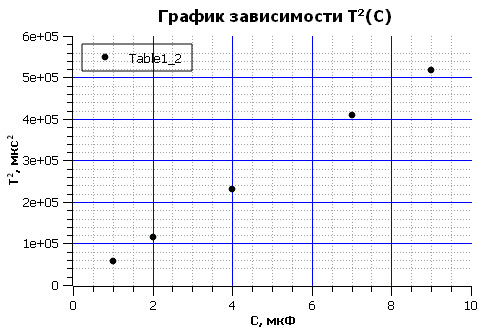
\includegraphics[scale = 1]{формулаТомсона.jpg}
	\end{figure}

	\noindent \textbf{Вывод:} график $T^2(C)$ представляет собой линейную зависимость, таким образом, приходим к выводу о справедливости формулы Томсона.
	
	\noindent Измерим зависимость логарифмического декремента затухания от сопротивления. 

	\begin{table} [h!]
		\begin{center}
			\begin{tabular}{|c|c|c|c|c|}
				\hline
				$R_{\text{внеш}}$, Ом  & $n$  & $U_1/U_n$ & $\theta$ & $Q$     \\ \hline
				0  & 23 & 2     & 0.03  & 104.6 \\ \hline
				2  & 21 & 2     & 0.033 & 95.15 \\ \hline
				4  & 20 & 2     & 0.034 & 92.35 \\ \hline
				6  & 19 & 2     & 0.036 & 87.22 \\ \hline
				8  & 17 & 2     & 0.041 & 76.59 \\ \hline
				10 & 25 & 3     & 0.044 & 71.36 \\ \hline
				12 & 24 & 3     & 0.046 & 68.26 \\ \hline
				15 & 28 & 4     & 0.049 & 64.08 \\ \hline
			\end{tabular}
		\end{center}
	\end{table}

	\noindent Вычислим теоретическое значение критического сопротивления.
	
	\begin{equation*}
		R_{\text{кр}} = 2 \sqrt{\frac{L}{C}} = 2 \sqrt{\frac{143.47 \cdot 10^{-3}}{2 \cdot 10^{-8}}} \approx  5356.68 \text{Ом}
	\end{equation*}
	
	\begin{equation}
		\theta = \gamma T = \frac{R}{2 L} 2 \pi \sqrt{L C} = R \pi \sqrt{\frac{C}{L}} = \frac{2 \pi}{R_{\text{кр}}}R
	\end{equation}
	
	\begin{equation}
		R = R_{\text{внеш}} + R_{\text{внутр}}
	\end{equation}
	
	\begin{equation}
		\theta = \frac{2 \pi}{R_{\text{кр}}} R_{\text{внеш}} + \frac{2 \pi}{R_{\text{кр}}} R_{\text{внутр}}
	\end{equation}
	
	\noindent Построим график зависимости $\theta(R)$ и выразим $R_{\text{внеш}}$ $R_{\text{внутр}}$.
	
	\begin{figure}[h!]
		\centering
		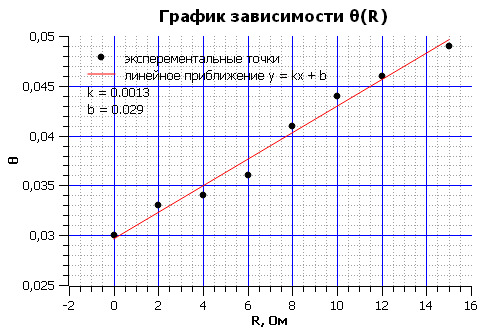
\includegraphics[scale = 1]{дикримент_сопротивление}
	\end{figure}
	
	\begin{equation*}
		\frac{2 \pi}{R_{\text{кр}}} = 0.0013 \Rightarrow R_{\text{кр}} \approx 4830.77 ~ \text{Ом}
	\end{equation*}
	
	\begin{equation*}
		\frac{2 \pi}{R_{\text{кр}}} R_{\text{внутр}} = 0.029 \Rightarrow R_{\text{внутр}} \approx 22.31 ~ \text{Ом}
	\end{equation*}
	
	\noindent \textbf{Вывод:} таким образом, с помощью графика зависимости $\theta(R)$ мы нашли значения внутреннего и критического сопротивления.
	
	\noindent Вычислим логарифмический декремент затухания по фазовой диаграмме.\\
	
	\begin{figure} [h!]
		\centering
		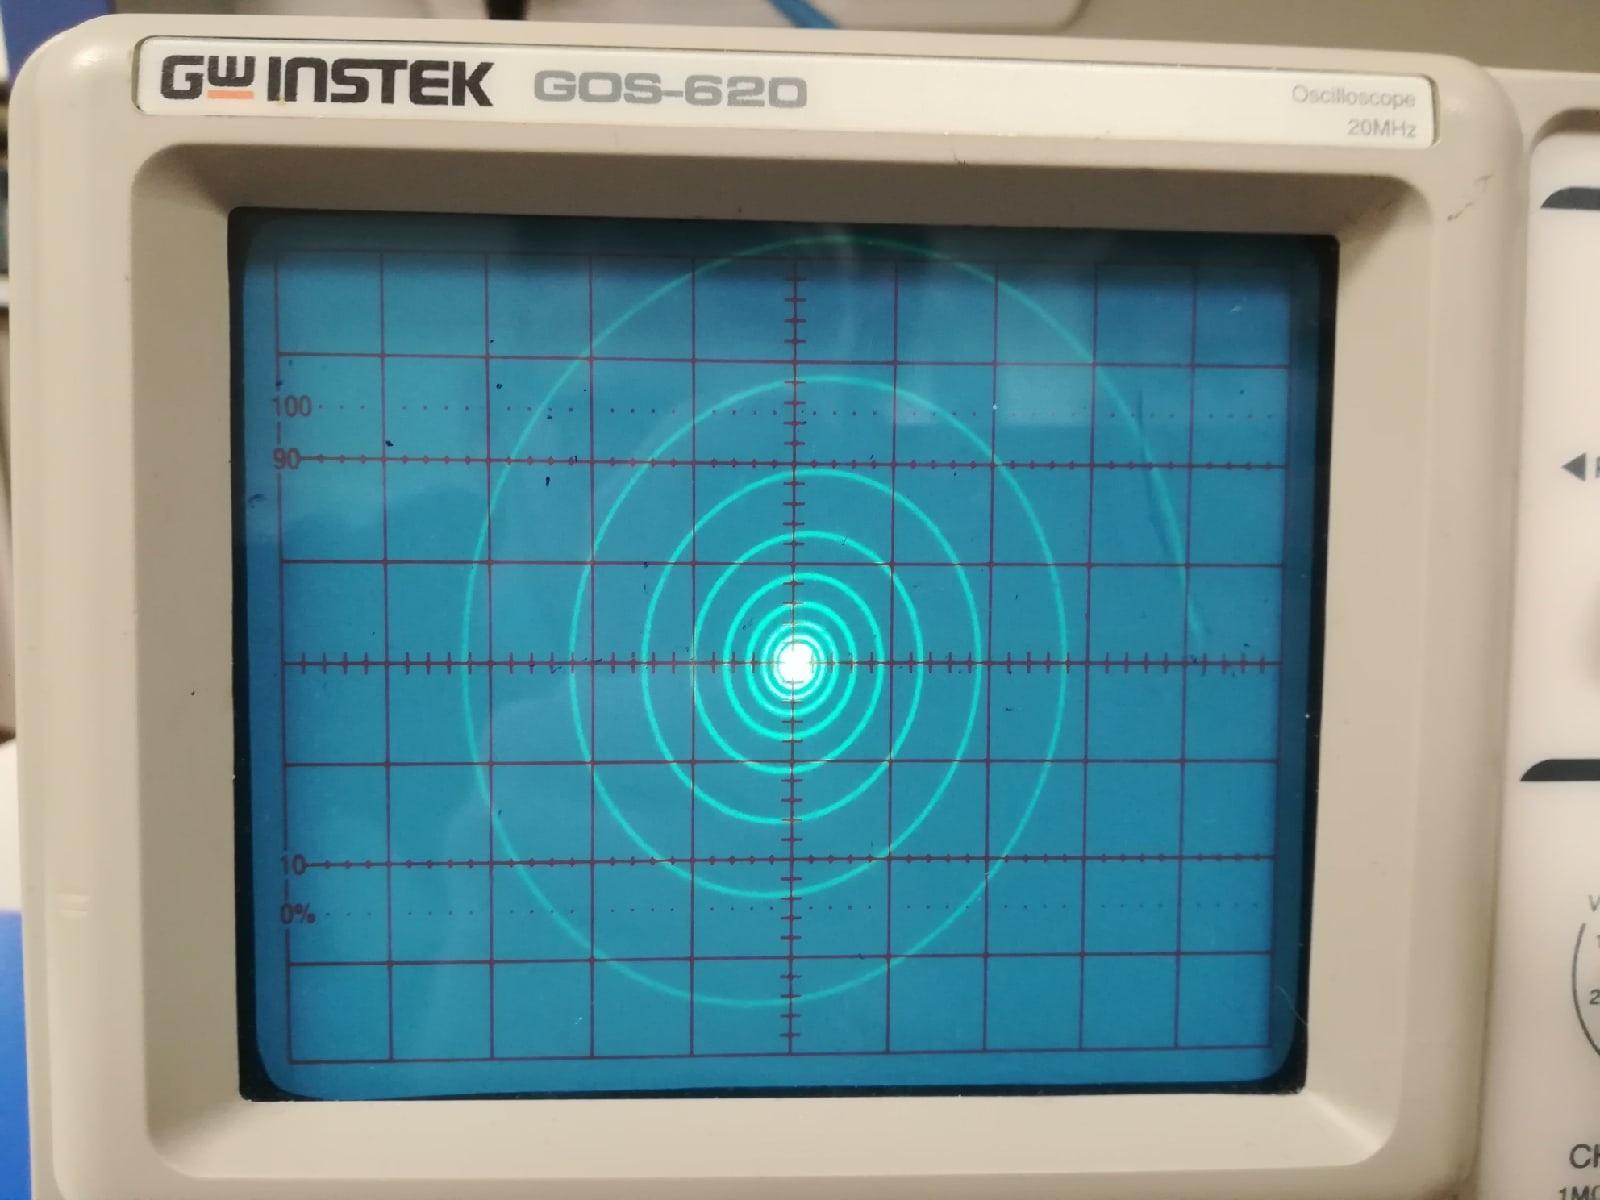
\includegraphics[scale = 0.16]{фазовая_диаграмма_рис1.jpg}
		\caption{Колебания на фазовой диаграмме R = 300 Ом}
	\end{figure}
	
	\begin{figure} [h!]
		\centering
		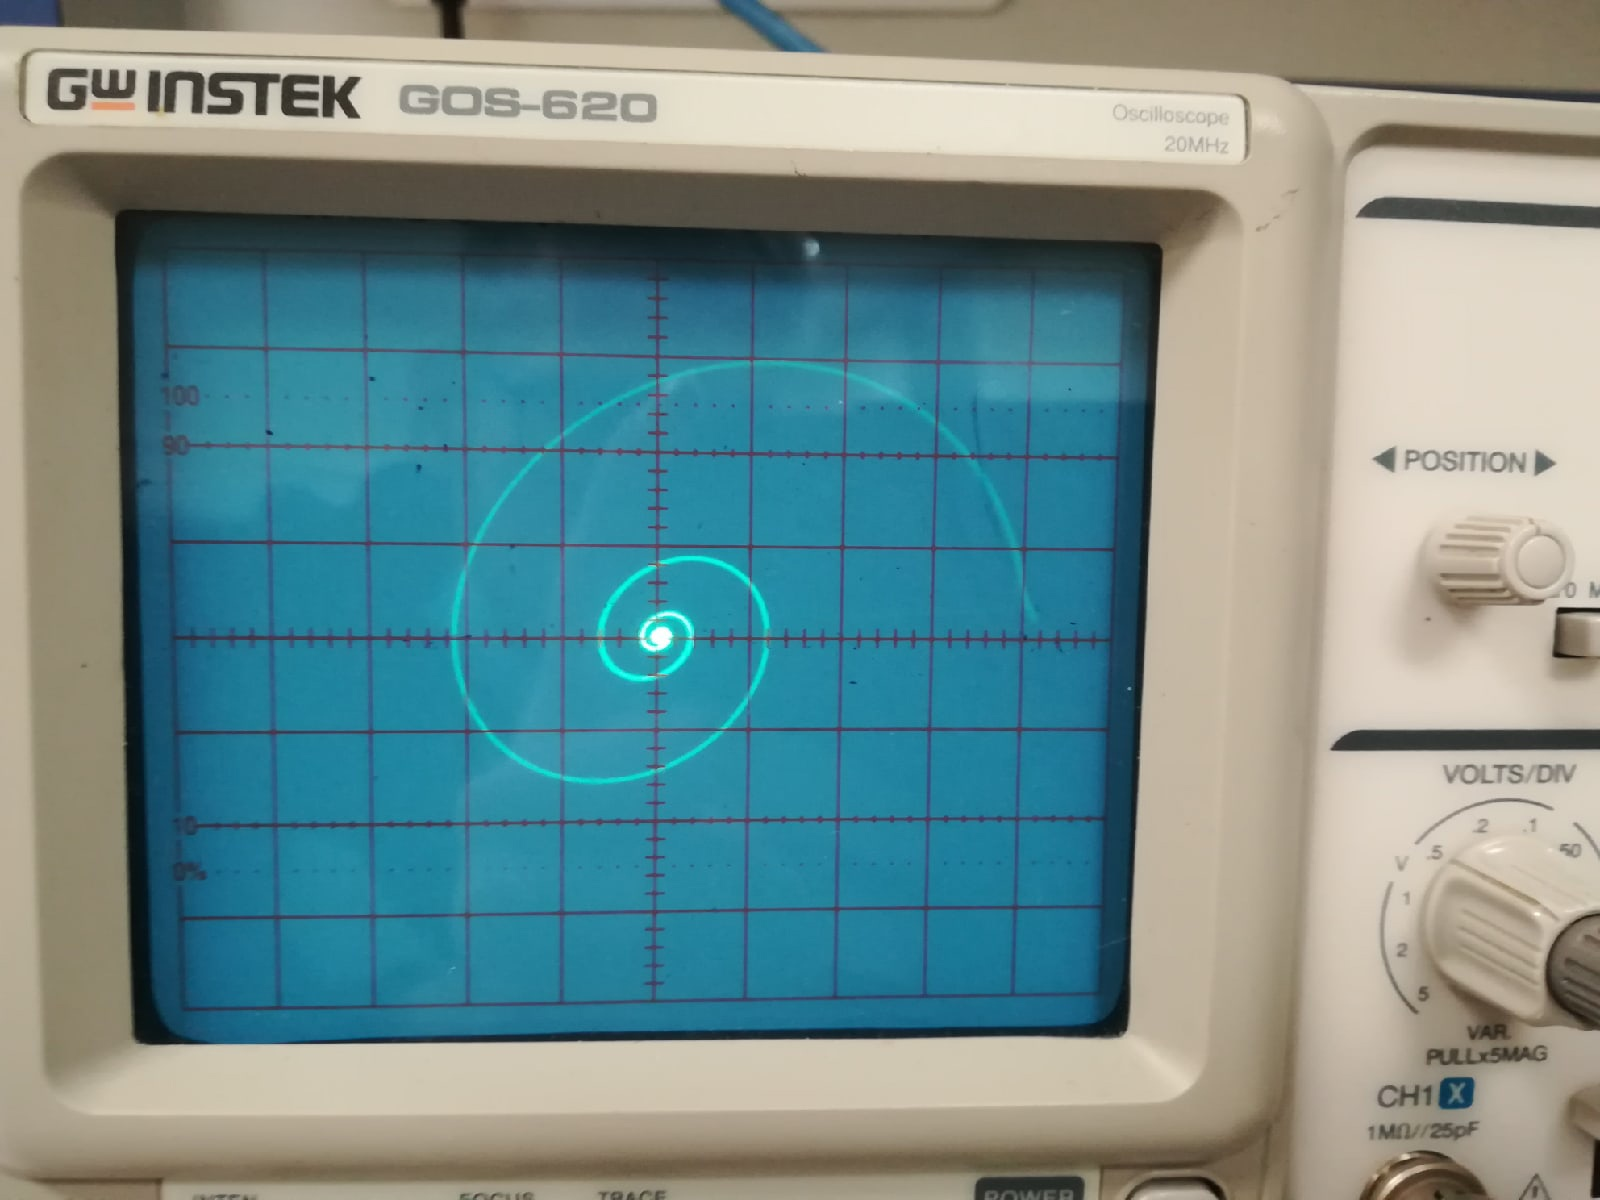
\includegraphics[scale = 0.16]{фазовая_диаграмма_рис2.jpg}
		\caption{Колебания на фазовой диаграмме R = 1 кОм}
	\end{figure}

	%\newpage

	\noindent Вычисления выполним по формуле:
	
	\begin{equation}
		\Theta = \frac{1}{n} \ln \frac{U_k}{U_{k + n}}
	\end{equation}
	
	\[ 300 ~ \text{Ом:} ~ \theta = \frac{1}{4} \ln \frac{14}{3} \approx 0.39 \]
	
	\[ 1 ~ \text{кОм:} ~ \theta = \ln \frac{6}{2} \approx 1.09 \]
	
\end{document}




